\chapter{Optimal Investment with Proportional Transaction Costs}
%\section{Introduction}

%%%%%%%%%%%%%%%%%%%%%%%%%%%%%%%%%%%%%%%%%%%%%%%%%%%%%%%%%%%%%%%%%%%%%%%%%%
%\begin{comment}
The problem of optimal portfolio management of securities was first formulated by Merton \cite{Merton}. It is known as Merton's porfolio problem or the consumption-investment problem. It concerns a question how to allocate wealth between consumption and investment in order to maximize expected utility over a time horizon. This general problem can be considered under numerous different specific formulations. For example, Merton derived analytical solution for the problem with two assets under logarithmic utility function over both finite and infinite horizon. %However under many formulations the analytical solution is not known or does not even exist. In these cases we are forced to use numerical methods.

In this section we consider the problem with proportional transaction costs as formulated in \cite{Dostal}. We summarize the dynamics of the model and propose its approximation by Markov chain. Then we use the algorithm from the Chapter 1 to solve the problem. The results are compared with analytical solution. 

%he problem when there are transaction costs from assets trading, received a considerable reasearch atention in recent years. The article \cite{survey} provides a survey on this literature. We will use iterative algorithm, derived in the Chapter 1, to provide a numerical solution of the problem formulated in Bielicky, Chancelier, Pliska, Sulem \cite{Benchmark} and Bielicky, Pliska \cite{Benchmark2}.
%\end{comment}
%%%%%%%%%%%%%%%%%%%%%%%%%%%%%%%%%%%%%%%%%%%%%%%%%%%%%%%%%%%%%%%%%%%%%%%%%%

%Under many set-ups the f solution is not known. 
%formulation is reather general and  and must allocate his wealth between stocks and a risk-free asset maximize utility over a 
%Optimal asset allocation problem\\
%Briefly describe: set-up, criterion, strategy...\\

\section{Model description} 
Suppose that a market consists of two assets. The first one is assumed to be riskless and the second one is assumed to be risky. Time development of the riskless asset, denoted by $S^0$, is deterministic and is given by
\begin{equation}
\mathrm{d}S^0_t=r\,S^0_t\,\mathrm{d}t.
\end{equation}
This asset represents a bank account with constant interest rate $r$ and with continuous compounding. Starting with a certain deposit the account grows exponentially in time with growth rate equal to $r$.

The second asset, denoted by $S^1$, represents a stock or a stock index. We assume that it's price follows geometric Brownian motion with drift $\mu$ and volatility $\sigma$. That is
\begin{equation}
\mathrm{d}S^1_t=\mu\,S^1_t\mathrm{d}t+\sigma\,S^1_t\,\mathrm{d}W_t,
\end{equation}
where $W_t$ is a Brownian motion. 
%The other option is to keep the money in the bank account. For simplicity we assume that the bank account do not earn any interest. 
We assume that no other assets are available.%, so a potential investor can invest only in these two assets.

Further we assume that both assets, the stock and the money, are infinitely divisible. % and no short selling is allowed. 
So the investor can possess any non-negative real volumes of these assets.

As mentioned in the introduction, the transaction costs are paid when trading the risky asset. These transaction costs are proportional to the size of the deal. In case of buying a $(1+c_{+})$ - multiple of the stock price is paid. On the other hand, in case of selling, $(1-c_{-})$ - multiple of the stock price is received. We consider $c_{+}\in(0,\infty)$ and $c_{-}\in(0,1)$.

%%%%%%%%%%%%%%%%%%%%%%%%%%%%%%%%%%%%%%%%%%%%%%%%%%%%%%%%%%%%%%%%%%%%%%%%%%
\begin{comment}
For simplicity we assume that the costs do not distinguish between buying and selling. That is for both operations the transaction costs are the same. Formally, if the investor buys (or sells) $\Delta N^1_t$ amount of stocks at time $t$, he pays transaction costs equal to  
\[c\,S^1_t|\Delta N^1_t|\,.\]
The constant $c$ represents transaction costs per deal of a unit size. 
Because every rebalancing of the porfolio bears transaction costs, it is reasonable to expect that the investor will not trade continuously in time but in discrete time instants.  Thus we restrict possible strategies to the ones given by a sequence $(\tau_k,N_k)$, $k\in\mathbb{N}$. The variables $\tau_k$ determine the time instants, when the investor rebalances portfolio. The variable $N_k$, which obtains values from the interval $[0,\infty)$, represents the number of stocks in portfolio immediately after the transaction is realized in time $\tau_k$. Of course at the time of decision making the future price development of risky asset is not known. Only the information known prior to the time of a decision making can be used. Formally, the strategy must satisfy
\begin{enumerate}
\item $\tau_k$ is $\mathcal{F}_t=\sigma(S_s^1,s\leq t)$ stopping time,
\item $N_k$ is $\mathcal{F}_{\tau_k}$ measurable variable.
\end{enumerate}
%Times $\tau_k$ determines the time instants, when the investor rebalances portfolio. Only informations until can be used, no crystal ball. 
Strategies of the form described above are called {\em pure impulse} strategies. 
Remind that we also made assumption, that no extra money can be poured into the portfolio. 
%Thus the number of stock after transaction must satisfy constrain condition insuring value neutrality of the portfolio.
So the portfolio must satisfy value neutrality condition. For the number of stocks after the $k$-th transaction $N_k$ it means that
\[N_{k-1}\cdot S^1_{\tau_k}-c\,S_{\tau_k}\,(N_k^1-N^1_{k-1})=N_k\cdot S_{\tau_k}.\]
%Further impose rather technical condition, that the value of the portfolio must allways must have positive value 
%\[N_k\cdot S_{\tau_k} > 0.\]
Having a pure inpulse strategy $(\tau_k,N_k)$, $k\in\mathbb{N}$, we can construct the process determining number of risky assets in the portfolio in every time instance $t$. This process is given by
\[ N_t:=N_k \quad \text{for}\quad t\in[\tau_k,\tau_{k+1}), \quad k\in\mathbb{N}, \quad t\in\mathbb{R}.\]
Here we commit a slight abuse of language. While $N$ indexing by natural numbers means number of risky assets in times of trading, $N$ indexing by real numbers means number of risky assets in any time instance.
\end{comment}
%%%%%%%%%%%%%%%%%%%%%%%%%%%%%%%%%%%%%%%%%%%%%%%%%%%%%%%%%%%%%%%%%%%%%%%%%%

\begin{comment}
the following risk-sensitive performance criterion to evaluate certain strategy,
\begin{equation}
\label{criterion}
J_{\gamma}=\liminf_{t\rightarrow\infty}\tfrac{1}{\gamma}t^{-1}\log\mathbb{E}[V_t^{\gamma}].
\end{equation}

It follows that the objective is to find a strategy that maximizes $J_{\gamma}$. %trade such that optimally according to the following risk-sensitive criterion
This criterion provides the trade-off between a portfolio's exponential growh rate and its asymptotic variance. Moreover, the bigger the value of the parameter $\gamma$, the more risk averse the investor is. For further analysis of the criteria, please see \cite{Benchmark2} %Interpretaion of criterion...
\end{comment}
We will consider a utility function with hyperbolic absolute risk aversion (HARA) of the form
\begin{equation}
\label{HARAutility}
\mathcal{U}^{\texttt{H}}_{\gamma}(x)=\tfrac{1}{\gamma}\,x^{\gamma}, \quad \gamma<0.
\end{equation}
%The parameter $\gamma$ represents risk sensitivity.

The aim of the investor is to maximize the growth rate of the certainty equivalent of the value of the portfolio. That is to maximize 
\begin{equation}
\label{criteria}
\lim_{t\rightarrow\infty}t^{-1}\log(\texttt{CE}_{\gamma}^{\texttt{H}}(V_t)),\quad \texttt{CE}_{\gamma}^{\texttt{H}}(V_t):=(\mathcal{U}^{\texttt{H}}_{\gamma})^{-1}\,\mathbb{E}\,\mathcal{U}^{\texttt{H}}_{\gamma}(V_t),
\end{equation}
where $V_t$ is the value of the portfolio at time $t$.

There is an important relation \eqref{CHrelation} between HARA utility function and CARA utility function from the first Chapter, which can be easily shown by direct computation.
\begin{equation}
\label{CHrelation}
\texttt{CE}_{\gamma}^{\texttt{C}}(\log(\cdot))=\log(\texttt{CE}_{\gamma}^{\texttt{H}}(\cdot)).
\end{equation}
According to \eqref{CHrelation}, the criteria \eqref{criteria} can be reformulated as
\begin{equation}
\label{CHcriteria}
\lim_{t\rightarrow\infty}t^{-1}\log(\texttt{CE}_{\gamma}^{\texttt{H}}(V_t)) =\lim_{t\rightarrow\infty}t^{-1}\texttt{CE}_{\gamma}^{\texttt{C}}(\log(V_t)).
\end{equation}
The relation \eqref{CHcriteria} coverts the problem of maximizing \eqref{criteria} to the problem we considered in the chapter one. The main benefit of this conversion is that we can work with $\log(V_t)$ instead of $V_t$. As we will see further, $\log(V_t)$ behaves better for purpose of approximation.

%The idea is to analytically derive the dynamics of the portfolio and then, using approximative Markov chain, find the optimal control. 
Now we analytically derive the dynamics of the portfolio. First we look at the dynamics of the value of the portfolio investment. Denote the number of riskless and risky assets in the portfolio at time $t$ by $N^0_t$ and $N^1_t$ respectively. The value of the portfolio at time $t$ is given by
\[V_t=N\tr_t\!S_t = N^0_t \, S^0_t + N^1_t \, S^1_t.\]
If the investor does not trade, number of both assets $N^0_t$, $N^1_t$ remains constant. Then we can write 

\begin{align*}
\mathrm{d}V_t &=N_t^0\,\mathrm{d}S_t^0+N_t^1\mathrm{d}S_t^1\\
&=N_t^0\,r\,S_t^0\mathrm{d}t + N_t^1(\,\mu\,S_t^1\mathrm{d}t + \sigma\,N_t^0\,r\,S_t^1\mathrm{d}W_t)\\
&=r \,V_t\,\frac{N^0_t\,S_t^0}{N\tr_t\!S_t}\,\mathrm{d}t+\mu\,V_t\,\frac{N^1_t\,S_t^1}{N\tr_t\!S_t}\,\mathrm{d}t
  +\sigma\,V_t\,\frac{N^1_t\,S_t^1}{N\tr_t\!S_t}\,\mathrm{d}W_t.
%&=r \,V_t\,\frac{N^0_t\,S_t^0}{N_t^0\,S_t^0 + N_t^1\,S_t^1}\,\mathrm{d}t+\mu\,V_t\,\frac{N^1_t\,S_t^1}{N_t^0\,S_t^0 + N_t^1\,S_t^1}\,\mathrm{d}t +\sigma\,V_t\,\frac{N^1_t\,S_t^1}{N_t^0\,S_t^0 + N_t^1\,S_t^1}\,\mathrm{d}W_t.
\end{align*}
Defining
\begin{equation}
\label{Gdef}
G_t=\frac{N^1_t\,S_t^1}{N_t^0\,S_t^0 + N_t^1\,S_t^1},
\end{equation}
we gain
\begin{equation}
\label{qv}
\frac{\mathrm{d}V_t}{V_t}=[r+(\mu-r)\,G_t]\,\mathrm{d}t+\sigma\,G_t\,\mathrm{d}W_t.
\end{equation}
Note that the variable $G_t$ represents the portion of the investor's wealth that is hold in the risky asset. We would refer to this quantity as an investor's \textit{position}. The process $(G_t, t\geq0)$ attains only values from the interval $[0,1]$. This is particularly important, because later we would like to approximate this process by a Markov chain with finite state space. %and to use the results from the first chapter. 
This would be problematic in the case of unbounded state domain.

Using Ito's lemma we compute dynamics of the logarithm of the value of the portfolio. According to \eqref{qv} %the quadratic variation of the process  is equal to
\[V_t^{-1}\mathrm{d}\left\langle V\right\rangle_t=\sigma^2\,G_t^{2}\,\mathrm{d}t,\] 
and we have  %(\textit{add reference to stochastic calculus part}). 
\begin{equation}
\mathrm{d}\log V_t =\frac{\mathrm{d}V_t}{V_t}-\frac{\left\langle\mathrm{d}V\right\rangle_t}{2\,V_t^2}=[r+(\mu-r)\,G_t-\tfrac{1}{2}\sigma^2\,G_t^2 ]\,\mathrm{d}t+\sigma\,G_t\,\mathrm{d}W_t.
\end{equation}
For technical details of the above computation see Appendix D. Denote
\[q_0(x)=r+(\mu-r)\,x-\tfrac{1}{2}\sigma^2\,x^2.\]
Then we can write
\begin{equation}
\label{Vdynamics}
\mathrm{d}\log V_t=q_0(G_t)\,\mathrm{d}t+\sigma\,G_t\,\mathrm{d}W_t.%.-\nu_{\pm}(G_t)\mathrm{d}^{\pm} G_t.
\end{equation}  

We managed to derive the dynamics of $\log V_{t}$ in terms of $G_{t}$. Now we would like to compute the dynamics of $G_t$. %Since dynamics caused by trading is described by differentials $\mathrm{d}^{\pm} G_t$, we only need to derive the dynamics in case of no trading. 
Using Ito's formula we gain
\begin{equation*}
V_t\,\mathrm{d} V_t^{-1} = -\frac{\mathrm{d}V_t}{V_t}+\frac{(\mathrm{d}V_t)^2}{V_t^2}=[-r-(\mu-r)\,G_t+\sigma^2\,G_t^2]\,\mathrm{d}t -\sigma\,G_t\,\mathrm{d}W_t.
\end{equation*}
Once again, the details of the computation can be found in Appendix D. Realizing that $G_t=N_t^1\,S_t^1\,V_t^{-1}$, we compute

\begin{align*}
\mathrm{d} G_t&=N_t^1\,V_t^{-1}\,\mathrm{d}S_t^1+N_t^1\,S_t^1\,\mathrm{d}V_t^{-1}+N_t^1\,(\mathrm{d}S_t^1)\,(\mathrm{d}V_t^{-1})\\
&=N_t^1\,V_t^{-1}\,(\mu\,S_t^1\,\mathrm{d}t+\sigma\,S+t^1 \mathrm{d}W_t) + N_t^1\,S_t^1\,V_t^{-1}[(-r(\mu-r)\,G_t+\sigma^2\,G_t^2)\mathrm{d}t\\ 
&\quad -\sigma^2\,G_t\,\mathrm{d}W_t]-N_t^1\,V_t^{-1}\,\sigma^2\,G_t\,S_t^1\,\mathrm{d}t  \\
&=G_t(\mu\mathrm{d}t+\sigma\mathrm{d}W_t)+G_t[(-r-(\mu-r)\,G_t+\sigma^2\,G_t^2)\,\mathrm{d}t-\sigma\,G_t\,\mathrm{d}W_t]-\sigma^2\,G_t^2\,\mathrm{d}t\\
&=G_t(\mu-r-(\mu-r)\,G_t-\sigma^2\,G_t^2-\sigma^2\,G_t)\,\mathrm{d}t + G_t\,(\sigma-\sigma\,G_t)\,\mathrm{d}W_t\\
&=G_t\,(1-G_t)[(\mu-r-\sigma^2\,G_t)\,\mathrm{d}t + \sigma\,\mathrm{d}W_t].
\end{align*}
%For the sake of simplicity of notation we define functions describing drift and volatility,
Define functions describing drift and volatility
\[b(x)=x\,(1-x)\,(\mu-r-\sigma^2\,x),\]
\[s(x)=\sigma\,x\,(1-x).\]
Now we can express the dynamics of $G_t$ as
\begin{equation}
\label{position}
\mathrm{d}G_t=b(G_t)\mathrm{d}t+s(G_t)\mathrm{d}W_t.%-\mathrm{d}^{\pm} G_t.
\end{equation}


%-------------------------------------------------\\
%{\color{red} TO DO}
In order to add trading to the dynamics, denote the sum of stocks bought and sold on the interval $[0,t)$ by $N_t^{+}$ and $N_t^{-}$ respectively. So the total number of stocks $N^1_t$ is equal to $N_t^{+} - N_t^{-}$. %\cite{Dostal}
%We assume that the trading can be realized only in discrete time instances. That is, the processes $N_t^{+}$ and $N_t^{-}$ have piecewise constant trajectories. Buying $\mathrm{d}N_t^{+}$ or selling $\mathrm{d}N_t^{-}$ amount of stocks bears transaction costs equal to $c_{\pm}\,S_t\,\mathrm{d}N_t^{\pm}$. Using Ito...see Dostal... Putting this to \eqref{qv} we get
Using Ito's lemma we can compute the dynamics of $G_t$ and $\log(V_t)$. The technical details are similar to the computations above. Here we only state the resulting differentials. For $G_t$ we get
\begin{equation}
\label{position}
\mathrm{d}G_t=b(G_t)\mathrm{d}t+s(G_t)\mathrm{d}W_t+\mathrm{d}^{+} G_t-\mathrm{d}^{-} G_t,
\end{equation}
where
\[\mathrm{d}^{+} G_t=\frac{(1+c_{+}\,G_t)\,S_t}{V_t}\,\mathrm{d}N_t^{+},\quad \mathrm{d}^{-} G_t= \frac{(1-c_{-}\,G_t)\,S_t}{V_t}\,\mathrm{d}N_t^{-}.\]
For $\log(V_t)$ we get
\begin{equation}
\label{VdynamicsCost}
\mathrm{d}\log V_t=q_0(G_t)\,\mathrm{d}t+\sigma\,G_t\,\mathrm{d}W_t-\nu_{+}(G_t)\mathrm{d}^{+} G_t-\nu_{-}(G_t)\mathrm{d}^{-} G_t,
\end{equation}
where
\begin{equation}
\label{mudef}
\nu_{+}(x)=\frac{c_{+}}{1+c_{+}\,x}, \quad \nu_{-}(x)=\frac{c_{-}}{1+c_{-}\,x}.
\end{equation}
%------------------------------------------------- 

%%%%%%%%%%%%%%%%%%%%%%%%%%%%%%%%%%%%%%%%%%%%%%%%%%%%%%%%%%%%%%%%%
\begin{comment}
What still holds is the fact that the investor trades in discrete time instants $\tau_k$, due to transaction costs. Transaction is realized instantly, so the prices of assets during the trade do not change. Thus the only effect on the portfolio value at time $\tau_k$ is a decline equal to transaction costs. That is 
\[V_{\tau_k}-V_{\tau_k-}=-c\,S^1_{\tau_k}\Delta N^1_{\tau_k}\]
Than for the change in logarithm of the value we have
%We compute (\textit{add detail})
\begin{equation}
%\Delta\log V_{\tau_k}=-|\Delta\ln(1+c\,G_{\tau_k})|.
\Delta\log V_{\tau_k}=\log \frac{V_{\tau_k}}{V_{\tau_k-}}=\log \frac{V_{\tau_k-}-c\,S^1_{\tau_k}|\Delta N^1_{\tau_k}|}{V_{\tau_k-}}=\log(1-c\,|\Delta G_{\tau_k}|).
\end{equation}
The total dynamics can be expressed as follows,
\begin{equation}
\label{lnV}
%f V_{\tau_k}=[r+(\mu-r)\,G_t-\tfrac{1}{2}\sigma^2\,G_t^2]\,\mathrm{d}t+\sigma\,G_t\,\mathrm{d}W_t-\sum_{k=0}^{\infty}\mathbb{I}_{[\tau_k\leq t]} |\Delta\ln(1+c\,G_{\tau_k})| 
\log V_{t}=V_0+\int_0^t[r+(\mu-r)\,G_s-\tfrac{1}{2}\sigma^2\,G_s^2]\,\mathrm{d}s+\int_0^t \sigma\,G_s\,\mathrm{d}W_s-\sum_{k=0}^{\infty}\mathbb{I}_{[\tau_k\leq t]} |\Delta\log(1+c\,G_{\tau_k})|.
\end{equation}
%Having 
We managed to derive dynamics of $\log V_{t}$ in terms of $G_{t}$. Now we would like to compute dynamics $G_t$. Since dynamics caused by trading is described by differentials $\mathrm{d}^{\pm} G_t$, we only need to derive the dynamics in case of no trading. Using Ito's formula we gain
\begin{equation*}
V_t\,\mathrm{d} V_t^{-1} = -\frac{\mathrm{d}V_t}{V_t}+\frac{(\mathrm{d}V_t)^2}{V_t^2}=[-r-(\mu-r)\,G_t+\sigma^2\,G_t^2]\,\mathrm{d}t -\sigma\,G_t\,\mathrm{d}W_t.
\end{equation*}
Once again, the technical details of the computation can be found in Appendix D. Realizing that $G_t=N_t^1\,S_t^1\,V_t^{-1}$, we compute
\begin{align*}
\mathrm{d} G_t&=N_t^1\,V_t^{-1}\,\mathrm{d}S_t^1+N_t^1\,S_t^1\,\mathrm{d}V_t^{-1}+N_t^1\,(\mathrm{d}S_t^1)\,(\mathrm{d}V_t^{-1})\\
&=N_t^1\,V_t^{-1}\,(\mu\,S_t^1\,\mathrm{d}t+\sigma\,S+t^1 \mathrm{d}W_t) + N_t^1\,S_t^1\,V_t^{-1}[(-r(\mu-r)\,G_t+\sigma^2\,G_t^2)\mathrm{d}t\\ 
&\quad -\sigma^2\,G_t\,\mathrm{d}W_t]-N_t^1\,V_t^{-1}\,\sigma^2\,G_t\,S_t^1\,\mathrm{d}t  \\
&=G_t(\mu\mathrm{d}t+\sigma\mathrm{d}W_t)+G_t[(-r-(\mu-r)\,G_t+\sigma^2\,G_t^2)\,\mathrm{d}t-\sigma\,G_t\,\mathrm{d}W_t]-\sigma^2\,G_t^2\,\mathrm{d}t\\
&=G_t(\mu-r-(\mu-r)\,G_t-\sigma^2\,G_t^2-\sigma^2\,G_t)\,\mathrm{d}t + G_t\,(\sigma-\sigma\,G_t)\,\mathrm{d}W_t\\
&=G_t\,(1-G_t)[(\mu-r-\sigma^2\,G_t)\,\mathrm{d}t + \sigma\,\mathrm{d}W_t].
\end{align*}
%For the sake of simplicity of notation we define functions describing drift and volatility,
Define functions describing drift and volatility
\[b(x)=x\,(1-x)\,(\mu-r-\sigma^2\,x),\]
\[s(x)=\sigma\,x\,(1-x).\]
Now we can express the dynamics of $G_t$ as
\begin{equation}
\label{position}
\mathrm{d}G_t=b(G_t)\mathrm{d}t+s(G_t)\mathrm{d}W_t-\mathrm{d}^{\pm} G_t.
\end{equation}
%The process $G_t$ is the one that will be approximated...\\
%\eqref{CHcriteria}
%cannot directly imply approach...change of measure.blbosti...\\
\end{comment}
%%%%%%%%%%%%%%%%%%%%%%%%%%%%%%%%%%%%%%%%%%%

Finally we look at dynamics of the utility $\mathcal{U}^{\texttt{H}}_{\gamma}(V_t)$, which should determine the rewards for our approximating chain. For sake of simplicity we will consider the dynamics without trading. First remind that
%be is essential part of our performance critera \eqref{criteria}. 
\begin{equation}
\label{eq21}
\mathcal{U}^{\texttt{H}}_{\gamma}(x)=\tfrac{1}{\gamma}\,x^{\gamma}=\gamma^{-1}\exp\{\gamma\log(V_t)\}.
\end{equation}
Using Ito's Lemma with $f(x)=\exp\{\gamma x\}$ and \eqref{Vdynamics} we get %Having the dynamics of value of the portfolio \eqref{Vdynamics} and the dynamics of the position \eqref{position}, we can derive the dynamicswe get
\begin{equation}
\label{eq22}
\begin{split}
\mathrm{d}\gamma^{-1}\exp\{\gamma \log(V_t)\}&=V_t^{\gamma}\,\mathrm{d}\log(V_t)+\tfrac{1}{2}\gamma\,V_t^{\gamma}\mathrm{d}\left\langle \log(V) \right\rangle_t\\
&=(V_t^{\gamma}\,q_0(G_t)+\tfrac{1}{2}\gamma\sigma^2 G_t^2) \mathrm{d}t + V_t^{\gamma}\sigma \mathrm{d}W_t\\
&=V_t^{\gamma}\,q_{\gamma}(G_t)\mathrm{d}t + V_t^{\gamma}\sigma \mathrm{d}W_t,\\
\end{split}
\end{equation}
where
\[q_{\gamma}(x)=q_{0}(x)+\tfrac{1}{2}\gamma\sigma^2 x^2.\]
Thus the expected utility of the value of the portfolio is
\[\mathbb{E}\,\mathcal{U}_{\gamma}(V_t)=\mathbb{E}\,\int_0^tV_s^{\gamma}\,q_{\gamma}(G_s)\mathrm{d}s.\]
The process $G$ is the one we would like to approximate by Markov chain. However, in order to determine the rewards for $G$, we need the expected utility  $\mathbb{E}\,\mathcal{U}_{\gamma}(V_t)$ to be dependent only on $G_t$. The Girsanov theorem (see Appendix D) can help us to get rid of dependence on $V_t$. Assume without loss of generality that $V_0=1$. Than by equation \eqref{Vdynamics} we can express $\mathcal{U}_{\gamma}(V_t)$ as 
%\begin{align}
\begin{equation*}
\begin{split}
\mathcal{U}_{\gamma}(V_t)&=\tfrac{1}{\gamma}\exp\{\gamma\log(V_t)\}\\
&=\gamma^{-1}\exp\Big\{\gamma\int_0^t q_0(G_s)\mathrm{d}s + \sigma\gamma \int_0^t G_s \mathrm{d}W_s \Big\}\\
&=\gamma^{-1}
\exp\Big\{\sigma\gamma \int_0^t G_s \mathrm{d}W_s -\tfrac{1}{2}\sigma^2\gamma\int_0^t G_s^2\mathrm{d}s\Big\}  \exp\Big\{\gamma\int_0^t q_\gamma(G_s)\mathrm{d}s\Big\}.\\
%&=\gamma^{-1}\,\mathcal{E}_t\,\exp\Big\{\gamma\int_0^t q_{\gamma}(G_s)\mathrm{d}s\Big\}
\end{split}
\end{equation*}
%\end{align}
Defining the stochastic exponential
\[\mathcal{E}(X)_t=\exp\{X_t-\tfrac{1}{2}\left\langle X\right\rangle_t\}, \quad X_t=\sigma\gamma\int_0^t G_s \mathrm{d}W_s,\]
we can write 

\begin{equation}
\mathcal{U}_{\gamma}(V_t)=\gamma^{-1}\,\mathcal{E}(X)_t\,\exp\Big\{\gamma\int_0^t q_{\gamma}(G_s)\mathrm{d}s\Big\}.
\end{equation}
Since $G_t$ attains only values in $[0,1]$, it satisfies Novikov condition,
\begin{equation}
\mathbb{E}\left[\exp\Big(\frac{1}{2}\int_0^t G^2_s \,\mathrm{d}s \Big)\right]<e^{\tfrac{t}{2}}<\infty, \quad t\geq0.
\end{equation}
Thus, we can use the Girsanov theorem \ref{Girsanov} which gives us existence of the measure $\mathbb{Q}_t$, absolutely continuous to the underlying measure $\mathbb{P}$, for which
\begin{equation}
\label{Qreward}
\begin{split}
\mathbb{E}_{\mathbb{P}}\,\mathcal{U}_{\gamma}(V_t)&=\mathbb{E}_{\mathbb{P}}\,\mathcal{E}(X)_t\exp\Big\{\gamma\int_0^t q_{\gamma}(G_s)\mathrm{d}s\Big\}\\
&=\mathbb{E}_{\mathbb{Q}_t}\,\exp\Big\{\gamma\int_0^t q_{\gamma}(G_s)\mathrm{d}s\Big\}.
\end{split}
\end{equation}
We see that by moving to the measure $\mathbb{Q}_t$ we get rid of dependence on $V$. The only thing that remains to derive is the dynamics of $G$ under the measure $\mathbb{Q}_t$. According to \ref{Girsanov}
\begin{equation}
\label{QBM}
\mathrm{d}W_s=\mathrm{d}\widetilde{W}_s+\left\langle W,X \right\rangle_s=\mathrm{d}\widetilde{W}_s+\gamma\sigma G_t\mathrm{d}t,
\end{equation}
where $\widetilde{W}_s$ is a standard Brownian motion under $\mathbb{Q}_t$ on the interval $[0,t]$. Putting \eqref{position} and \eqref{QBM} together we get

\begin{equation*}
%
\begin{split}
\mathrm{d}G_t&=b(G_t)\mathrm{d}t+s(G_t)\mathrm{d}W_t+\mathrm{d}^{+} G_t-\mathrm{d}^{-} G_t\\
&=b(G_t)\mathrm{d}t+s(G_t)(\mathrm{d}\widetilde{W}_t+\gamma\sigma G_t\mathrm{d}t)+\mathrm{d}^{+} G_t-\mathrm{d}^{-} G_t
\end{split}
\end{equation*}
So the dynamics of $G_t$ under the $\mathbb{Q}$ is 
\begin{equation}
\label{Qposition}
\mathrm{d}G_t=\widetilde{b}(G_t)\mathrm{d}t+s(G_t)\mathrm{d}\widetilde{W}_t+\mathrm{d}^{+} G_t-\mathrm{d}^{-} G_t,
\end{equation}
where
\begin{equation}
\begin{split}
\widetilde{b}(x)&=b(x)+s(x)\,\gamma\,\sigma\,x\\
&=(1-\gamma)\,\sigma^2\,x\,(1-x)\,[\tfrac{(\mu-r)\,\sigma^2}{1-\gamma}-x].
\end{split}
\end{equation}



\begin{comment}
  \begin{equation*}
  \begin{split}
  \mathrm{d}\log Y_t&=q_0(G_t)\mathrm{d}t+\sigma G_t(\mathrm{d}\widetilde{W}_t+\gamma \sigma G_t      
  \mathrm{d}t)-\nu_{\pm}(G_t)\mathrm{d}^{\pm}G_t\\
   &=q_{\gamma}(G_t)\mathrm{d}t+\sigma G_t \mathrm{d}\widetilde{W}_t-\nu_{\pm}(G_t)\mathrm{d}^{\pm}G_t.
   \end{split}
   \end{equation*}
\end{comment}


%Note that every time the investor trades a stock, he changes the portion of the risky part of the portfolio $G_t$. Thus the trading strategy $(\tau_k,N_k)$ can be also expressed as $(\tau_k,G_k)$, where $G_k$ is portion of risky part immediately after transaction is realized at time $\tau_k$. In the following sections we work with this formulation of trading strategy. 
%Reformulation of pure impulse strategy in terms of $G_t$ missing
%%%%%%%%%%%%%%%%%%%%%%%%%%%%%%%%%%%%%%%%%%%%%%%%%%%%%%%%%%%%%%%%%%%%%%%%%%%%%%%%%%%%%%%%%%%%%%%%%%%%%%%%%%%%%%%%%%%%%%%%%
\section{Analytical Solution}

%The optimal strategies in case of proportional transaction costs

Dost�l \cite{Dostal} derived analytical solution for the problem of maximizing \eqref{criteria}. The optimal strategy is not to trade if the position $G_t$ is in certain interval $[\alpha,\beta]$, and to buy or sell the stock in order to keep the position within the interval $[\alpha,\beta]$. Dost�l shows that, considering a \textit{interval strategy} $[\alpha,\beta]$, the certainty equivalent growth rate can be computed as %He consider the interval strategies. That is the strategies as the optimal stragy are of this form keep position in the interval $(\alpha,\beta)$ Considering the interval He showed that

\begin{equation}
\lim_{t\rightarrow\infty}t^{-1}\log(\texttt{CE}^{\texttt{H}}(V_t))=\tfrac{\sigma^2}{2} u(\alpha,\beta),
\end{equation}

where the function $u(\alpha,\beta)$ is defined as the unique solution to the equation
\begin{equation}
\label{IntegralEquation}
\log\frac{1/\alpha-1}{1/\beta-1}=\int_{\xi_{-}(\beta)}^{\xi_{+}(\alpha)}\frac{dz}{\gamma z^2 +2\rho z - u(\alpha,\beta)},
\end{equation}
where 
\[\rho=\frac{\mu}{\sigma^2}-\frac{1}{2}, \quad\ \xi_{-}(x)=x\frac{1-c_{-}}{1-c_{-} x}, \quad \xi_{+}(x)=x\frac{1+c_{+}}{1+c_{+} x}.\]
The optimal interval strategy can be found by maximizing the function $u(\alpha,\beta)$ over $\{(\alpha,\beta):\alpha,\beta\in(0,1),\alpha<\beta\}$.
Unfortunately, the equation \ref{IntegralEquation} do not have a closed-form solution, so the optimization must be carried out numerically.

\section{Discrete Time Approximation}

%{\em interval strategy only}

We will approximate the continuous time model from previous section by discrete time Markov chain. Methods we use are based on monograph \cite{KushnerDupuis}. For further detail see chapters 4 and 5 in this monograph. %(\textit{ciation, "all that is important..."})
The key requirement for approximating Markov chain is that it must preserve the basic characteristics of original process, namely conditional mean and conditional variance.

As we mentioned earlier we will approximate the position process $G$ under the measure $\mathbb{Q}$, which is given by the equation \eqref{Qposition}. First we look at the model without trading. Investor's trading decisions or, in terminology of the first chapter, investor's actions, will be added later. Approximation in both time and state domain are needed. In order to do this we create a lattice on which the approximating chain will be allowed to move. Let us start with time domain. Let $0=t_0<t_1<t_2\dots$ be the sequence with step $t_k-t_{k-1}=\Delta t$, which is the same for all $k$. The change of characteristics of the original process in time step $\Delta t$ can be approximated according to \eqref{Qposition} as follows%Then the characteristics of the original process can be approximated as follows
\begin{equation}
\label{EOrg}
\mathbb{E}[G_{t_k+1}-G_{t_k}|G_{t_k}=g]\sim \widetilde{b}(g) \Delta t,
\end{equation}
\begin{equation}
\label{VarOrg}
\text{var}[G_{t_k+1}-G_{t_k}|G_{t_k}=g]\sim\mathbb{E}[(G_{t_k+1}-G_{t_k})^2|G_{t_k}=g]\sim s^{2}(g)\Delta t.
\end{equation}
In case of conditional variance we neglect the second order term %(\textit{ref. to stoch. calc.})
\[(\mathbb{E}[(G_{t_k+1}-G_{t_k})|G_{t_k}=g])^2\sim (\widetilde{b}(g))^2\,(\Delta t)^2,\]
which is acceptable for small enough $\Delta t$.

Now we move to approximation in state domain of $G_t$, which is the interval $[0,1]$. Let $\{g_i\}_{i=1}^{n}$ be the equidistant partition of the interval $[0,1]$ with the norm equal to $\delta=\tfrac{1}{n}$. The set $\{g_i\}_{i=1}^{n}$ will be the state space of the approximating Markov chain. We denote this chain by $\widehat{G}=(\widehat{G}_k,k\in\mathbb{N})$. Suppose the $\widehat{G}$ is in state $g$. Denote the probability that it moves to the state $g+h$ by  $P_{+}(g)$ and the probability that it moves to the state $g-h$ by  $P_{-}(g)$. The probability that the chain stays in $g$ in the next step is denoted $P_{0}(g)$. We will not allow probability of moving to the other states to be positive. %This is reasonable for small enough time step $\Delta t$. %(\textit{return to this question later}) 
Of course these probabilities must satisfy
\[P_0(g)=1-P_{+}(g)-P_{-}(g).\]
First we need to compute moment characteristics of the chain in term of these probabilities. Then we can determine values $P_{+}(g)$, $P_{-}(g)$ and $P_{0}(g)$ by comparison with characteristics of the original process. We obtain
\begin{align*}
\mathbb{E}[\widehat{G}_{k+1}|\widehat{G}_{k}=g]&=P_{-}(g)\,(g-\delta)+P_{0}(g)\,g+P_{+}(g)\,(g+\delta)\\
&=g-P_{-}(g)\,\delta+P_{+}(g)\,\delta.
\end{align*}
Subtracting $\widehat{G}_{k}=g$ we gain
\begin{equation}
\label{EDis}
\mathbb{E}[\widehat{G}_{k+1}-\widehat{G}_{k}|\widehat{G}_{k}=g]=\delta(P_{+}(g)-P_{-}(g)),
\end{equation}
\begin{equation}
\label{VarDis}
\begin{split}
\text{var}[\widehat{G}_{k+1}-\widehat{G}_{k}|\widehat{G}_{k}=g]&\sim\mathbb{E}[(\widehat{G}_{k+1}-\widehat{G}_{k})^2|\widehat{G}_{k}=g]\\
&\sim \delta^2(P_{+}(g)+P_{-}(g)).
\end{split}
\end{equation}
When we compare \eqref{EOrg} with \eqref{EDis} and \eqref{VarOrg} with \eqref{VarDis} we gain the following equations

\begin{equation}
\begin{split}
\label{EqSustava}
b(g)\Delta t&= \delta(P_{+}(g)-P_{-}(g)),\\
\\
s^2(g)\Delta t&= \delta^2(P_{+}(g)+P_{-}(g)).
\end{split}
\end{equation}
Solving the equations \eqref{EqSustava} we get

\begin{equation*}
P_{+}(g)=\frac{\delta\,\widetilde{b}(g)+s^2(g)}{2\delta^2}\,\Delta t,%\geq0
\end{equation*}

\begin{equation*}
P_{-}(g)=\frac{-\delta\,\widetilde{b}(g) t+s^2(g)}{2\delta^2}\,\Delta t.%\geq0
\end{equation*}
From \eqref{EqSustava} also immediately follows that
\begin{equation*}
P_0(g)=1-P_{+}(g)-P_{-}(g)=1-\frac{s^2(g)\Delta t}{\delta^2}.
\end{equation*}
%Back to choice of disretization steps.. 
Nonnegativity of $P_0(g)$ gives us the constraint $s^2(g)\Delta t\leq \delta^2$. We can choose the time step $\Delta t$ such that
\[\Delta t=\frac{\delta^2}{k},\]
where $k\geq s^2(g)$ holds for every state $g$.

Now we add actions to the chain, meaning trading decisions. We consider three types of actions: action $+$ means to buy stocks, action $-$ means to sell stocks and action $0$ means to do nothing. For the states close to extreme points, not all decisions are allowed. The set of all admissible actions depending on state $A_g$ are as following:  

\begin{itemize}
  \item $A_{0}=\{+\}$, $A_{1}=\{-\}$: in the extreme points only one decision is allowed in order to push  back inside the interval $(0,1)$, 
  \item $A_{h}=\{+,0\}$, $A_{1-h}=\{0,-\}$: only decisions that keep the position inside the interval $(0,1)$ are allowed,
  \item $A_{g}=\{+,0,-\}$, $g=2h,3h\dots,1-2h$: in the rest of the states all alternatives are possible.
\end{itemize}

As we derived above, in case of action $0$, the transition probabilities are following
\begin{align*}
&\qquad p_{i,i-1}=P_{-}(g_i),\\
(0):&\qquad p_{i,i}=P_{0}(g_i),\\
&\qquad p_{i,i+1}=P_{+}(g_i).
\end{align*}
%\begin{comment}
  
  In case of buying or selling, we left the small probability $\epsilon>0$ that the decision is not realized, in   order to keep the chain irreducible. So if the decision to buy is realized the chain $\widehat{G}$ is shifted up. So, the transition probabilities looks like
  \begin{align*}
  &\qquad (1-\epsilon)\,P_{-}(g_{i+1}) \text{ in case of transition } i+1 \rightarrow i,\\
  (+):i\rightarrow i+1&\qquad (1-\epsilon)\,P_{0}(g_{i+1}) \text{ in case of transition } i+1 \rightarrow i+1,\\
  &\qquad (1-\epsilon)\,P_{+}(g_{i+1}) \text{ in case of transition } i+1 \rightarrow i+2.
  \end{align*}
  In case that decision to buy is not realized the transition probabilities looks like
  \begin{align*}
  &\qquad \epsilon\,P_{-}(g_{i}) \text{ in case of transition } i \rightarrow i-1,\\
  (+):i\rightarrow i&\qquad \epsilon\,P_{0}(g_{i}) \text{ in case of transition } i \rightarrow i,\\
  &\qquad \epsilon\,P_{+}(g_{i}) \text{ in case of transition } i \rightarrow i+1.
  \end{align*}
  Putting altogether, we have
  \begin{align*}
  &\qquad p_{i,i-1}=\epsilon\,P_{-}(g_i),\\
  (+):&\qquad p_{i,i}=\epsilon\,P_{0}(g_i)+(1-\epsilon)\,P_{-}(g_{i+1}),\\
  &\qquad p_{i,i+1}=\epsilon\,P_{+}(g_i)+(1-\epsilon)\,P_{0}(g_{i+1}),\\
  &\qquad p_{i,i+2}=(1-\epsilon)\,P_{+}(g_{i+1}).
  \end{align*} 
  Similarly for decision to sell we get
  \begin{align*}
  &\qquad p_{i,i-2}=(1-\epsilon)\,P_{-}(g_{i-1}),\\
  &\qquad p_{i,i-1}=(1-\epsilon)\,P_{0}(g_{i-1})+\epsilon\,P_{-}(g_{i}),\\
  (-):&\qquad p_{i,i}=(1-\epsilon)\,P_{+}(g_{i-1})+\epsilon\,P_{0}(g_{i}),\\
  &\qquad p_{i,i+1}=\epsilon\,P_{+}(g_{i}).
  \end{align*}
%\end{comment}
\begin{comment}
Decision to buy risky asset shifts the chain $\widehat{G}$ up. So the transition probabilities look like  
\begin{align*}
&\qquad p_{i,i}=P_{-}(g_i),\\
(+):&\qquad p_{i,i+1}=P_{0}(g_i),\\
&\qquad p_{i,i+2}=P_{+}(g_i).
\end{align*} 
Similarly for selling decision we have transition probabilities
\begin{align*}
&\qquad p_{i,i-2}=P_{-}(g_i),\\
(-):&\qquad p_{i,i-1}=P_{0}(g_i),\\
&\qquad p_{i,i}=P_{+}(g_i).
\end{align*} 
\end{comment}
For any given control we have defined Markov chain $\{\widehat{G}_n\}_{n=0}^{\infty}$ that approximates the original process $\{G_t,t\geq0\}$. 
Denote rewards in case of actions $0$, $+$ and $-$ by $r_0$, $r_+$ and $r_-$ respectively. According to discrete time analogue of  the equation \eqref{Qreward}, we define rewards in case of no trading
\begin{equation*}
r_0(g_i)=q_\gamma(g_i)\,\Delta t =(r-(\mu-r)\,g_i+\tfrac{1}{2}(1-\gamma)\sigma^2\,g_i^2)\,\Delta t
\end{equation*}
Trading bears a costs given by \eqref{mudef}. Thus we define the rewards in case of trading as
\begin{eqnarray*}
r_+(g_i)&=&r_0(g_i)-\delta\,\nu_{+}(g_i)=r_0(g_i)-\delta\,c_{+}\,(1+c_{+} g_i)^{-1},\\	
r_-(g_i)&=&r_0(g_i)-\delta\,\nu_{-}(g_i)=r_0(g_i)-\delta\,c_{-}\,(1-c_{-} g_i)^{-1}.	 
\end{eqnarray*}

\begin{comment}
 The aim is to find strategy that maximizes
 \begin{equation}
 \label{criterionDiscr}
 J_{\gamma}=\lim_{n\rightarrow\infty}\tfrac{1}{\gamma}n^{-1}\log\mathbb{E}[\widehat{V}_n^{\gamma}],
 \end{equation}
 which is nothing else than discrete version of the criterion \eqref{criterion}. Recall that in the Chapter 1 we   developed iterative algorithm which finds a strategy that maximizes 
 \[\lim_{n\rightarrow\infty}\tfrac{1}{\gamma}n^{-1}\log\mathbb{E}[\exp\{-\gamma\,r(\widehat{V}_n)\}],\] 
 where $r$ is a reward function (compare with equation \eqref{CritCh1}). Notice that if we choose $\log(\cdot)$ for  our reward function, we get exactly criterion \eqref{criterionDiscr}. As a result, all we need to do is to define the rewards to the Makrov decision chain $\widehat{G}$ according to the dynamics of $\log(V_t)$. We have already derived dynamics of $\log(V_t)$ in Section 2.2. So based on equation \eqref{lnV}, we can define rewards for the chain  $\widehat{G}_n$. Denote rewards in case of actions $0$, $+$ and $-$ by $r_0$, $r_+$ and $r_-$ respectively. Then a  discrete time analogue of the equation \eqref{lnV}, gives us
\begin{equation*}
r_0(g_i)=(r-(\mu-r)\,g_i+\tfrac{1}{2}\sigma^2\,g_i^2)\,\Delta t
\end{equation*}
and
\begin{equation*}
\begin{split}
r_+(g_i)=r_-(g_i)&=r_0(g_i)-|\Delta\,\log(1+c\,g_i)|\\
								 &=r_0(g_i)-|\log(1+c\,g_i)-\log(1+c\,g_{i+1})|.
\end{split}
\end{equation*}
Here the reward is not paid for transition from one state to another but for staying in a particular state for an amount of time $\Delta t$. In this case (see section 1.3) the rewards are described by a reward vector $\bm{r}$  rather than a reward matrix. For example, if the strategy is given by a vector $(+,\cdots,+,0,\cdots,0,-,\cdots,-)$ than the reward vector is $(r_+,\cdots,r_+,r_0,\cdots,r_0,r_-,\cdots,r_-)$.

We have defined both the transition probabilities and the rewards, that means, the discrete time Markov decision chain is fully determined.

\begingroup
\renewcommand*{\arraystretch}{0.8}
  \begin{equation}
    \begin{pmatrix}
 r_+(g_1) & r_+(g_1) & r_+(g_1)       			              															\\
      		& \ddots & \ddots & \ddots              															\\
       &  & r_+(g_k) & r_+(g_k) & r_+(g_k) & &\multicolumn{2}{c}{\text{\kern0.5em\smash{\raisebox{-1ex}{\Large 0}}}}\\
          &        & r_0(g_{k+1})    & r_0(g_{k_1})    & r_0(g_{k+1})																			\\
          &        &        & \ddots & \ddots & \ddots    											\\  
          &        &        &        & r_0(g_l)    & r_0(g_l)    & r_0(g_l)    	 							\\     
          &  \multicolumn{2}{c}{\text{\kern-0.5em\smash{\raisebox{0.75ex}{\Large 0}}}} & &  & r_-(g_{l_1})    & r_-(g_{l_1})    & r_-(g_{l_1}) \\
          &        &        &        &        & \ddots & \ddots & \ddots    		\\  
          &        &        &        & 				&				 & r_-(g_n)    & r_-(g_n)    & r_-(g_n)  \\
    \end{pmatrix}
  \end{equation}
\endgroup
\end{comment}

%%%%%%%%%%%%%%%%%%%%%%%%%%%%%%%%%%%%%%%%%%%%%%%%%%%%%%%%%%%%%%%%%%%%%%%%%%%%%%%%%%%%%%%
\section{Continuous Time Approximation}

In this section, we approximate the model given in \eqref{Qposition} by continuous time Markov Chain. In that case time domain of the original process and the approximating chain are the same, thus only the of approximation in the state domain is needed. Similarly to previous section, we start with derivation of change in moment characteristics. Due to continuity of the time domain, we focus on the infinitesimal change.

\begin{equation}
\label{EOrgC}
\mathbb{E}[\underbrace{G_{t+\mathrm{d}t}-G_t}_{\mathrm{d}G_t}|G_{t}=g]= b(g)\,\mathrm{d}t
\end{equation}

\begin{equation}
\label{VarOrgC}
\text{var}[\mathrm{d}G_t|G_{t}=g]\sim\mathbb{E}[\mathrm{d}G_t^2|G_{t}=g]= s^{2}(g)\,\mathrm{d}t.
\end{equation}
Here we neglect the second order term %(\textit{ref. to stoch. calc.})
\[(\mathbb{E}[\mathrm{d}G_t|G_{t}=g])^2= (b(g))^2\,(\mathrm{d}t)^2.\]

Consider the same approximation of the state space $[0,1]$ as in previous section. That is the partition $\{g_i\}_{i=1}^{n}$ with the norm equal to $\delta$. We denote the continuous time approximating chain by $\widetilde{G}=(\widetilde{G}_t,t\geq0$). Further we denote the transition rate from any state $g$ to $g+\delta$ by $Q_+$ and the transition rate from state $g$ to $g-\delta$ by $Q_-$. We will not allow the other rates to be positive. So, for the total rate out of state $g$, denoted by $Q_0$, the equation $Q_0 + Q_+ + Q_- =0$ holds. Note that, according to Kolmogorov backward differential equation \eqref{KE}, for $t$ close to zero, we have the following differential relation between transition rates and transition probabilities
\[\mathrm{d}\bm{P}_t=\bm{Q}\,\bm{P}_{0}\,\mathrm{d} t=\bm{Q}\,\mathrm{d}t.\]
Using this, the infinitesimal change in mean value of the chain $\widetilde{G}$ can be expressed as
\begin{equation}
\label{EDisC}
\begin{split}
\mathbb{E}[\mathrm{d}\widetilde{G}_{t}|\widetilde{G}_{t}=g]&=\mathrm{d}P_{-}(g)\,(g-\delta)+\mathrm{d}P_{0}(g)\,g+\mathrm{d}P_{+}(g)\,(g+\delta)\\
&=[Q_{-}(g)\,(g-\delta)+Q_{0}(g)\,g+Q_{+}(g)\,(g+\delta)]\,\mathrm{d}t\\
&=[\delta(Q_{-}(g)+Q_{+}(g))]\,\mathrm{d}t
\end{split}
\end{equation}
Neglecting the second order term, we can express change in variance
\begin{equation}
\label{VarDisC}
\begin{split}
\text{var}[\mathrm{d}\widetilde{G}_{t}|\widetilde{G}_{t}=g]&\sim\mathbb{E}[(\mathrm{d}\widetilde{G}_{t})^2|\widetilde{G}_{t}=g]\\
&=[Q_{-}(g)\,(g-\delta)^2+Q_{0}(g)\,g^2+Q_{+}(g)\,(g+\delta)^2]\,\mathrm{d}t\\
%&\sim\mathbb{E}[(\widehat{G}_{k+1}-\widehat{G}_{k})^2|\widehat{G}_{k}=g]\\
&\sim [\delta^2(Q_{+}(g)+Q_{-}(g))]\,\mathrm{d}t.
\end{split}
\end{equation}
Comparing \eqref{EOrgC} with \eqref{EDisC}, and \eqref{VarOrgC} with \eqref{VarDisC} we gain the following equations
\begin{equation}
\label{EqSustavaC}
\begin{split}
b(g)&= \delta(Q_{+}(g)-Q_{-}(g)),\\
\\
s^2(g)&= \delta^2(Q_{+}(g)+Q_{-}(g)).
\end{split}
\end{equation}
Solving the equations \eqref{EqSustavaC} we get
\begin{equation*}
Q_{+}(g)=\frac{\delta\,b(g)+s^2(g)}{2\delta^2}\geq0,
\end{equation*}
\begin{equation*}
Q_{-}(g)=\frac{-\delta\,b(g)+s^2(g)}{2\delta^2}\geq0,
\end{equation*}
From \eqref{EqSustavaC} immediately follows that
\begin{equation*}
Q_0(g)=-Q_{+}(g)-Q_{-}(g)=-\frac{s^2(g)}{\delta^2}.
\end{equation*}
Again consider the same set of admissible actions $\mathcal{U}=\{+,-,0\}$ as in previous section. As we derived above, in case of non-trading (action $0$), the transition rates as follows
\begin{align*}
&\qquad q_{i,i-1}=Q_{-}(g_i),\\
(0):&\qquad q_{i,i}=Q_{0}(g_i),\\
&\qquad q_{i,i+1}=Q_{+}(g_i).
\end{align*}
In case of trading we would like the chain to move immediately from the current state. The immediate shift would be accomplished by infinite transition rate. However, for the finite state continuous chain the infinite rates are not allowed. Thus, we are forced to choose some large $K>0$, which will represent the intensity out of a state in case of trading. So, for a decision to buy we have
 \begin{align*}
&\qquad q_{i,i-1}=Q_{-}(g_i),\\
(+):&\qquad q_{i,i}=Q_{0}(g_i)-K,\\
&\qquad q_{i,i+1}=Q_{+}(g_i)+K,
\end{align*}
and for decision to sell we have
\begin{align*}
&\qquad q_{i,i-1}=Q_{-}(g_i)+K,\\
(-):&\qquad q_{i,i}=Q_{0}(g_i)-K,\\
&\qquad q_{i,i+1}=Q_{+}(g_i).
\end{align*}

%As in discrete time case we defined the rewards for the chain based on the equation \eqref{lnV}.
For continuous time Markov chain we distinguish reward for staying in a state and reward for transition from one state to another. The reward for staying in a state $g_i$ is described by \eqref{Qreward}. Thus we define  %$\bm{r}=\{r(g_i)\}$
\begin{equation*}
r(g_i)=q_\gamma(g_i)=(r-(\mu-r)\,g_i+\tfrac{1}{2}(1-\gamma)\sigma^2\,g_i^2).
\end{equation*}
This reward does not depend on decision taken in state $g_i$. The reward for transition from one state to another is related to a transaction cost. So these rewards occur only in case of trading assets, that is only in case of decision $+$ or $-$. According to \eqref{mudef} we have
\begin{eqnarray*}
r_+(g_i)&=&\nu_{+}(g_i)=-c_{+}\,(1+c_{+} g_i)^{-1},\\	
r_-(g_i)&=&\nu_{-}(g_i)=-c_{-}\,(1-c_{-} g_i)^{-1}.
\end{eqnarray*}
All the other transition rewards are equal to zero. 

%%%%%%%%%%%%%%%%%%%%%%%%%%%%%%%%%%%%%%%%%%%%%%%%%%%%%%%%%%%%%%%%%%%%%%%%%%%%%%%%%%%
\newpage
\section{Numerical results}

%Keep the partion $G$ in certain interval...
We implemented both discrete time and continuous time approximation of the model. Using the policy iteration algorithm developed in the first chapter we derive the optimal interval strategy according to the performance criteria \eqref{criteria}. We compare the results with analytical solution.

Remind that the analytical solution is not of the closed-form. It is given as the maximum of the function $u(\alpha,\beta)$, which is defined by integral equation \eqref{IntegralEquation}. We find the maximum approximately by evaluating the function $u$ on the discrete lattice $\{(a,b):0<a<b<1,a=n\,\delta, b=m\,\delta\}$ with the step $\delta=0.005$.

For both discrete time and continuous time approximation we choose the step in the state domain approximation $\delta=0.005$. In case of discrete time approximation we choose the step in the time space approximation $\Delta t=10^{-4}$.



\begin{table}[ht!]
%\vspace{5pt}
    \caption{Results comparison}
    \begin{center}
        \subtable[$\mu=0.5$] %
            { \footnotesize
              %\scriptsize
             \begin{tabular}{l | c  c}
              %\hline
                   &  $g$  & interval \\ \hline
               Cont. model & $0.056373$ & $(0.170, 0.335)$\\ 
               Discr. appr. & $0.056364$ & $(0.165, 0.335)$\\
               Cont. appr. & $0.056375$ & $(0.165, 0.335)$\\  %\hline
              
              \end{tabular}  
            }
        \hspace{1cm}    
        \subtable[$\mu=0.9$] %
            { \footnotesize
              %\scriptsize
              \begin{tabular}{l | c  c}
              %\hline
                   &  $g$  & interval \\ \hline
               Cont. model & $0.193513$ & $(0.350, 0.550)$\\ 
               Discr. appr. & $0.193490$ & $(0.355, 0.550)$\\
               Cont. appr. & $0.193510$ & $(0.355,0.550)$\\ %\hline
              
              \end{tabular}              
          }
    
        \label{table}
    \end{center}
    
\end{table}

The table \ref{table} shows the results of continuous model and both of its approximations. The certainty equivalent growth rates $g$ and corresponding optimal interval strategies are compared. We consider transaction costs $c_+=c_-=0.02$, interest rate $r=0$, volatility of the stock $\sigma=1$ and $\gamma=-1$. The cases (a) and (b) differs by choice drift of the stock $\mu$. We observed a sufficient consistency of both approximations with analytical solution.

\newpage
The figures 2.1 and 2.2 shows the iterations for discrete time approximation and continuous time approximation respectively. The left-hand side figures show the development of certainty equivalent growth rate. We see that each iteration improves the strategy. The right-hand figures show the development of the strategy.

%As it has been mentioned, due to transaction costs we restrict our consideration on pure impulse strategies, that is trading in discrete time instances. It turns out, as might be expected, that the optimal strategy is to keep the risky portion of portfolio value within certain inteval.  

%In the figure \ref{Contour}, we compare discrete time and continuous time approximation. Here we do not use iterative algorithms, we focus merely on approximation. We consider only strategies which keep the process $G$ in certain interval. A point in the graph represents an interval $I\subset[0,1]$ given by its center (horizontal axis) and its radius (vertical axis). For every such interval we computed the utility growth rate by finding a corresponding Perron-Frobenius eigenvalue. The lighter the color is, the bigger utility growth rate is. We see that both approximations lead to a very similar map and to the same optimal interval. In both cases the state domain approximation step $h$ is equal $0.25$, which leads to the total number $121$ of possible intervals. Computation of utility growth rate for all intervals takes several tens of minutes. (risk adjusted growth rate)

%We see that finding the optimal strategy by brute force is very time consuming. For finer approximation it will be certainly untractable. The iterative algorithms are much faster. The figure \ref{Devel} shows the iterations for both discrete time (upper two figures) and continuous time (lower two figures) cases. The left hand side figures shows the development of risk adjusted growth rate. We see that each itteration improves the strategy. The right hand figures show the development of strategy. In each iteration we are allowed to choose from all possible strategies. However in each step the resulting strategy was of the interval form. The speed allows us to use state domain approximation step $h$ to be equal $0.01$, with computing time within several minutes.  The discrete time algorithm needed $14$ iterations to find the optimal strategy, continuous time alghorithm needed only $9$ iterations to find (the same) result. This means that we needed to find Peeron-Frobenius eigenvalue, which is the most time consuming computation, only $14$ ($9$) times. This is a rapid improvement compared to the brute force method.

\begin{figure}[ht!]
\centering
\subfigure[Growth rate of \texttt{CE}, $\mu=0.5$.]{
   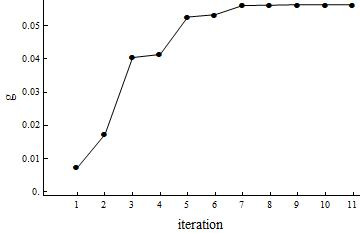
\includegraphics[scale =0.55] {DiscrApprox_G5.jpg}
   \label{GDevelDiscr}
 }
 \subfigure[Optimal strategy, $\mu=0.5$.]{
   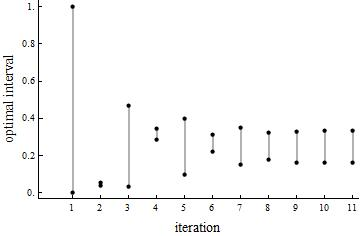
\includegraphics[scale =0.55] {DiscrApprox_Int5.jpg}
   \label{IDevelDiscr}
 }
  \subfigure[Growth rate of \texttt{CE}, $\mu=0.9$.]{
   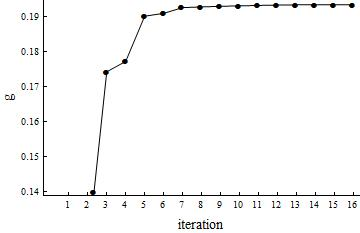
\includegraphics[scale =0.55] {DiscrApprox_G9.jpg}
   \label{GDevelCont}
 }
  \subfigure[Optimal strategy, $\mu=0.9$]{
   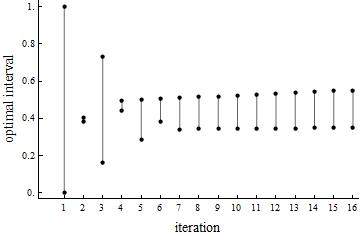
\includegraphics[scale =0.55] {DiscrApprox_Int9.jpg}
   \label{IDevelCont}
 }
\label{DiscrDevel}
\caption{Discrete time approximation, process of finding the optimal strategy.} %the parameters are $\mu=17$, $c=0.01$, $r=0.025$, $\sigma=0.5$ and $\gamma=1$.}
\end{figure}

\begin{figure}[ht!]
\centering
\subfigure[Growth rate of \texttt{CE}, $\mu=0.5$.]{
   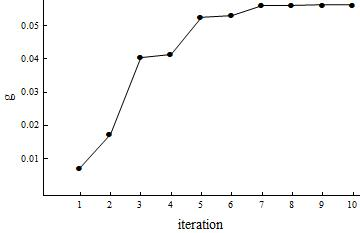
\includegraphics[scale =0.55] {ContApprox_G5.jpg}
   \label{GDevelDiscr}
 }
 \subfigure[Optimal strategy, $\mu=0.5$.]{
   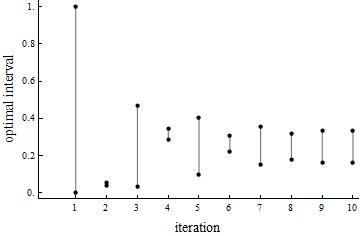
\includegraphics[scale =0.55] {ContApprox_Int5.jpg}
   \label{IDevelDiscr}
 }
  \subfigure[Growth rate of \texttt{CE}, $\mu=0.9$.]{
   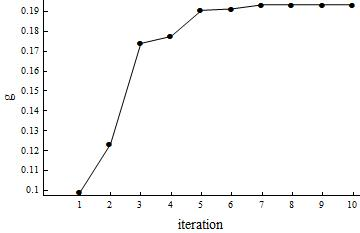
\includegraphics[scale =0.55] {ContApprox_G9.jpg}
   \label{GDevelCont}
 }
  \subfigure[Optimal strategy, $\mu=0.9$]{
   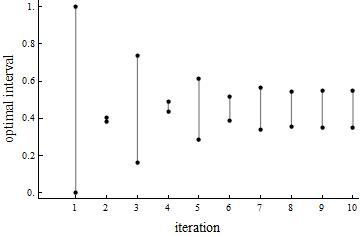
\includegraphics[scale =0.55] {ContApprox_Int9.jpg}
   \label{IDevelCont}
 }
\label{ContDevel}
\caption{Continuous time approximation, process of finding the optimal strategy.} %the parameters are $\mu=17$, $c=0.01$, $r=0.025$, $\sigma=0.5$ and $\gamma=1$.}
\end{figure}

\newpage

%Finally, we examine the dependance of optimal strategy on parameters of the model. We vary one parameter with the rest of the parameters fixed and we look at how the optimal interval changes. The figure \ref{Compr} shows the dependance on drift $\mu$, interest rate $r$, transaction costs $c$ and volatility $\sigma$ respectively. All the dependencies are in accordance with intuition. The higher is the drift, the more likely is the investor to hold his wealth in risky asset, so the optimal interval moves up. Opposite relation hold for interest rate $r$. With higher transaction cost the optimal interval becomes wider, which in consequence means less trading. With higher volatility of the risky asset the investor tends sharply to riskless asset.

\begin{comment}


\begin{figure}[ht]
\centering
\subfigure[]{
   \includegraphics[scale =0.45] {ComparativeMu.jpg}
   \label{ComprMu}
 }
 \subfigure[]{
   \includegraphics[scale =0.45] {ComparativeR.jpg}
   \label{ComprR}
 }
  \subfigure[]{
   \includegraphics[scale =0.45] {ComparativeC.jpg}
   \label{ComprC}
 }
  \subfigure[]{
   \includegraphics[scale =0.45] {ComparativeSigma.jpg}
   \label{ComprSigma}
 }
\label{Compr}
\caption{Dependance of optimal strategy on the parameters of the model, the fixed values of parameters are $\mu=17$, $c=0.01$, $r=0.025$, $\sigma=0.5$ and $\gamma=1$.}
\end{figure}
\end{comment}

%\chapter*{Conclusion}

%%%%%%%%%%%%%
%trading dynamics podla stanikovaj
\begin{comment}
\[V_t+b N^1_t S^1_t=V_t(1+c_{+} G_t)\]
remains the same before and after the transaction. In differential form we can write
\[\mathrm{d}^+ \log V_t=-\mathrm{d}^+\log(1+c_{+} G_t)=-\nu_+(G_t)\mathrm{d}^+ G_t,\]
where $\mathrm{d}^+$ represents the infinitesimal change caused by buying the stock and
\begin{equation}
\label{nuplus}
\nu_+(x)=\frac{c_{+}}{1+c_{+} x}.
\end{equation}
On the other hand if the investor sell the stock the quantity 
\[V_t-c N^1_t S^1_t=V_t(1-c_{-} G_t)\]
remains the same before and after the transaction. In differential form we can write
\[\mathrm{d}^- \log V_t=-\mathrm{d}^-\log(1-c_{-} G_t)=-\nu_-(G_t)\mathrm{d}^- G_t,\]
where $\mathrm{d}^-$ represents the infinitesimal change caused by buying the stock and
\begin{equation}
\label{numinus}
\nu_-(x)=\frac{c_{-}}{1-c_{-} x}.
\end{equation}
\end{comment}


%%%%%%%%%%%%%%%%%%%%%%%%%%%%%%%%%%%%%%%%%%%%%%%%%%%%%%%%%%%%%%%%%%%%%%%%
\begin{comment}
Now we add trading to the dynamics. Denote by $N_t^{+}$ and $N_t^{-}$ the sum of stocks bought and sold on the interval $[0,t)$ respectively. So the total number of socks $N^1_t$ is equal to $N_t^{+} - N_t^{-}$. We assume that the trading can be realized only in discrete time instances. That is, the processes $N_t^{+}$ and $N_t^{-}$ have piecewise constant trajectories. Buying $\mathrm{d}N_t^{+}$ or selling $\mathrm{d}N_t^{-}$ amount of stocks bears transaction costs equal to $c_{\pm}\,S_t\,\mathrm{d}N_t^{\pm}$. Putting this to \eqref{qv} we get
\begin{equation}
\label{qvv}
\mathrm{d}V_t=V_t\,[(r+(\mu-r)\,G_t)\,\mathrm{d}t+\sigma\,G_t\,\mathrm{d}W_t]-c_{+}\,S_t\,\mathrm{d}N_t^{+}+c_{-}\,S_t\,\mathrm{d}N_t^{-}.
\end{equation}

Using Ito's formula we gain
\begin{equation*}
V_t\,\mathrm{d} V_t^{-1} = -\frac{\mathrm{d}V_t}{V_t}+\frac{(\mathrm{d}V_t)^2}{V_t^2}=[-r-(\mu-r)\,G_t+\sigma^2\,G_t^2]\,\mathrm{d}t -\sigma\,G_t\,\mathrm{d}W_t + c_{\pm}\,V_t^{-1}\,\mathrm{d}^{\pm}N_t .
\end{equation*}
Once again, the technical details of the computation can be found in Appendix D. Realizing that $G_t=N_t^1\,S_t^1\,V_t^{-1}$, we compute {\color{red} (toto napisat prehladnejsie...)}

\begin{align*}
\mathrm{d} G_t&=(N_t^1\,V_t^{-1})\,\mathrm{d}S_t^1+(N_t^1\,S_t^1)\,\mathrm{d}V_t^{-1}+N_t^1\,(\mathrm{d}S_t^1)\,(\mathrm{d}V_t^{-1}) +(V_t^{-1}\,S_t^1)\mathrm{d}N_t^{\pm}\\
&=N_t^1\,V_t^{-1}\,(\mu\,S_t^1\,\mathrm{d}t+\sigma\,S+t^1 \mathrm{d}W_t) + N_t^1\,S_t^1\,V_t^{-1}[(-r(\mu-r)\,G_t+\sigma^2\,G_t^2)\mathrm{d}t+\\ 
&\quad -\sigma^2\,G_t\,\mathrm{d}W_t + c_{\pm}\,V_t^{-1}\,\mathrm{d}N_t^{\pm}] -N_t^1\,V_t^{-1}\,\sigma^2\,G_t\,S_t^1\,\mathrm{d}t +(V_t^{-1}\,S_t^1)\mathrm{d}N_t^{\pm} \\
&=G_t(\mu\mathrm{d}t+\sigma\mathrm{d}W_t)+G_t[(-r-(\mu-r)\,G_t+\sigma^2\,G_t^2)\,\mathrm{d}t-\sigma\,G_t\,\mathrm{d}W_t]-\sigma^2\,G_t^2\,\mathrm{d}t \\
&\quad c_{\pm}\,N_t\,S^1_t\,V_t^{-2}\,\mathrm{d}N_t^{\pm}+V_t^{-1}\,S_t^1\mathrm{d}N_t^{\pm}\\
&=G_t(\mu-r-(\mu-r)\,G_t-\sigma^2\,G_t^2-\sigma^2\,G_t)\,\mathrm{d}t + G_t\,(\sigma-\sigma\,G_t)\,\mathrm{d}W_t\\
&\quad +(1+c_{\pm}\,G_t)\,S_t\,V_t^{-1}\,\mathrm{d}N_t^{\pm}\\
&=G_t\,(1-G_t)[(\mu-r-\sigma^2\,G_t)\,\mathrm{d}t + \sigma\,\mathrm{d}W_t]+\mathrm{d}G_t^{\pm}.
\end{align*}
Define functions describing drift and volatility
\[b(x)=x\,(1-x)\,(\mu-r-\sigma^2\,x),\]
\[s(x)=\sigma\,x\,(1-x).\]
Now we can express the dynamics of $G_t$ as
\begin{equation}
\label{position}
\mathrm{d}G_t=b(G_t)\mathrm{d}t+s(G_t)\mathrm{d}W_t-\mathrm{d}^{\pm} G_t.
\end{equation}
\end{comment}

\addcontentsline{toc}{chapter}{\protect\numberline{}Conclusion}
\chapter*{Conclusion}

For both discrete time and continuous time Markov decision chains we developed the iterative algorithm for finding a control that maximizes
\begin{equation*}
\label{zaver}
\lim_{t\rightarrow\infty}\tfrac{1}{\gamma}\,t^{-1}\,\log(-\mathbb{E}[U_t]),
\end{equation*}
where $U_t$ is utility from reward over the time horizon $[0,t]$. The algorithm is numerically tractable. 

Both discrete time and continuous time version of algorithm were applied on a particular problem in portfolio optimization theory. It presents how a continuos time problem of optimal stochastic control can be solved numerically via Markov chain approximation. The method can be possibly applied for different problems. The results provide a sufficient consistency with the analytical solution, which demonstrate that they work properly.   

%demostrating a  for    in  works properly was applied

%The alghorthms was derive
%In the second chapter possible application of the alghorithm for continuous time problem was demostrated. By approximating 